\documentclass{standalone}

\usepackage{tikz}
\usetikzlibrary{calc}
\usetikzlibrary{arrows.meta}
\definecolor{col1}{RGB}{255,193,117}
\definecolor{col2}{RGB}{187,189,106}
\definecolor{col3}{RGB}{122,177,119}
\definecolor{col4}{RGB}{55,112,138}

\begin{document}
      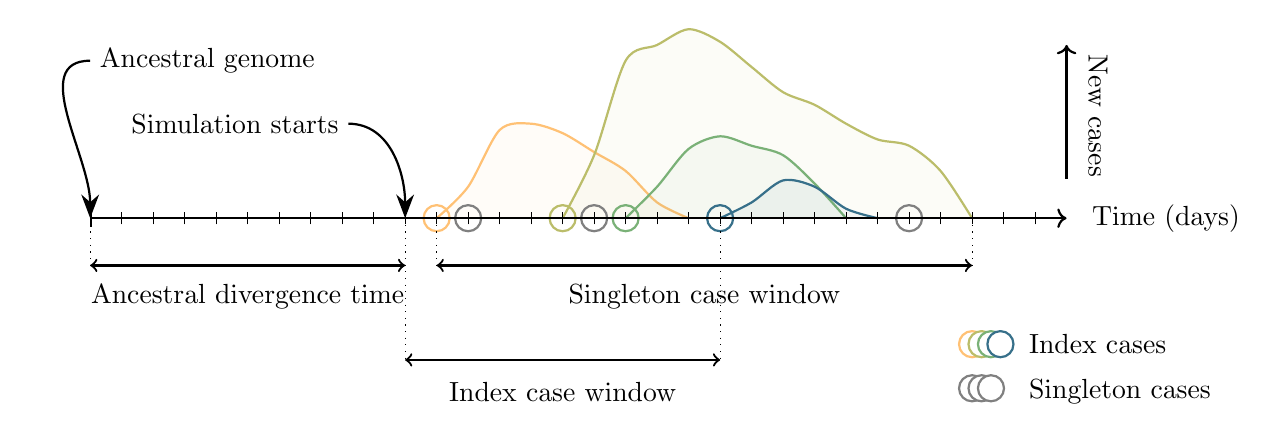
\begin{tikzpicture}[scale=0.4]
        \coordinate (origin) at (0, 0);
        
        \node (anclab) [anchor=west] at ($(origin) + (0, 5)$) {Ancestral genome};
        \draw[thick, -{Stealth[length=3mm]}] (anclab.west) to[out=180,in=90] (origin);
        
        \node (simlab) [anchor=west] at ($(origin) + (1, 3)$) {Simulation starts};
        \draw[thick, -{Stealth[length=3mm]}] (simlab.east) to[out=0,in=90] ($(origin) + (10, 0)$);
        
        \node [col1, thick, draw, circle] at ($(origin) + (11,0)$) {};
        \draw [col1, thick] plot [smooth] coordinates
            {(11,0) (12,1) (13,2.8) (14,3) (15,2.7) (16,2.1) (17,1.5) (18,0.5) (19,0)};
        \fill [col1, fill opacity = 0.05] plot [smooth] coordinates
            {(11,0) (12,1) (13,2.8) (14,3) (15,2.7) (16,2.1) (17,1.5) (18,0.5) (19,0)};
            
        \node [col2, thick, draw, circle] at ($(origin) + (15,0)$) {};
        \draw [col2, thick] plot [smooth] coordinates
            {(15,0) (16,2) (17,5) (18,5.5) (19,6) (20,5.6) (21,4.8) (22,4) (23,3.6) (24,3) (25,2.5) (26,2.3) (27,1.5) (28, 0)};
        \fill [col2, fill opacity = 0.05] plot [smooth] coordinates
            {(15,0) (16,2) (17,5) (18,5.5) (19,6) (20,5.6) (21,4.8) (22,4) (23,3.6) (24,3) (25,2.5) (26,2.3) (27,1.5) (28, 0)};
            
        \node [col3, thick, draw, circle] at ($(origin) + (17,0)$) {};
        \draw [col3, thick] plot [smooth] coordinates
            {(17,0) (18,1) (19,2.2) (20,2.6) (21,2.3) (22,2) (23,1.1) (24,0)};
        \fill [col3, fill opacity = 0.05] plot [smooth] coordinates
            {(17,0) (18,1) (19,2.2) (20,2.6) (21,2.3) (22,2) (23,1.1) (24,0)};
            
        \node [col4, thick, draw, circle] at ($(origin) + (20,0)$) {};
        \draw [col4, thick] plot [smooth] coordinates
            {(20,0) (21,0.5) (22,1.2) (23,1) (24,0.3) (25,0)};
        \fill [col4, fill opacity = 0.05] plot [smooth] coordinates
            {(20,0) (21,0.5) (22,1.2) (23,1) (24,0.3) (25,0)};
            
        \node [gray, thick, draw, circle] at ($(origin) + (12,0)$) {};
        \node [gray, thick, draw, circle] at ($(origin) + (16,0)$) {};
        \node [gray, thick, draw, circle] at ($(origin) + (26,0)$) {};
        
        \draw [dotted] (origin) -- +(0, -1.5);
        \draw [dotted] ($(origin) + (10,0)$) -- +(0, -4.5);
        \draw [dotted] ($(origin) + (11,0)$) -- +(0, -1.5);
        \draw [dotted] ($(origin) + (20,0)$) -- +(0, -4.5);
        \draw [dotted] ($(origin) + (28,0)$) -- +(0, -1.5);
            
        \draw [thick, to-to] ($(origin) + (10, -1.5)$) -- +(-10, 0);
        \node at ($(origin) + (5, -2.5)$) {Ancestral divergence time};
        
        \draw [thick, to-to] ($(origin) + (10, -4.5)$) -- +(10, 0);
        \node at ($(origin) + (15, -5.5)$) {Index case window};
        
        \draw [thick, to-to] ($(origin) + (11, -1.5)$) -- +(17, 0);
        \node at ($(origin) + (19.5, -2.5)$) {Singleton case window};
        
        \draw [thick,|->] (origin) -- +(31, 0);
        \foreach \i in {1,2,3,...,30} { \draw ($(origin) + (\i,-0.2)$) -- +(0,0.4); }
        \node [anchor=west] at ($(origin) + (31.5, 0)$) {Time (days)};
        
        \draw [thick,->] ($(origin) + (31, 1.25)$) -- +(0, 4.25);
        \node [rotate=270,anchor=east] at ($(origin) + (32, 1)$) {New cases};
        
        \node [anchor=west] at ($(origin) + (29.5,-4)$) {Index cases};
        \node [col1, thick, draw, circle, fill=white] at ($(origin) + (28,-4)$) {};
        \node [col2, thick, draw, circle, fill=white] at ($(origin) + (28.3,-4)$) {};
        \node [col3, thick, draw, circle, fill=white] at ($(origin) + (28.6,-4)$) {};
        \node [col4, thick, draw, circle, fill=white] at ($(origin) + (28.9,-4)$) {};
        
        \node [anchor=west] at ($(origin) + (29.5,-5.5)$) {Singleton cases};
        \node [gray, thick, draw, circle, fill=white] at ($(origin) + (28,-5.4)$) {};
        \node [gray, thick, draw, circle, fill=white] at ($(origin) + (28.3,-5.4)$) {};
        \node [gray, thick, draw, circle, fill=white] at ($(origin) + (28.6,-5.4)$) {};
      \end{tikzpicture}
\end{document}
